\documentclass[10pt]{beamer}
\usepackage[latin1]{inputenc}
\usepackage[T1]{fontenc}
\usetheme{metropolis}
\usepackage{appendixnumberbeamer}

\usepackage{booktabs}
\usepackage[scale=2]{ccicons}

\usepackage{pgfplots}
\usepgfplotslibrary{dateplot}


\usepackage{xspace}
\definecolor{mygreen}{rgb}{0,0.6,0}
\definecolor{mygray}{rgb}{0.5,0.5,0.5}
\definecolor{mymauve}{rgb}{0.58,0,0.82}
\usepackage{listings}
\lstset{ %
  backgroundcolor=\color{white},   % choose the background color; you must add \usepackage{color} or \usepackage{xcolor}; should come as last argument
  basicstyle=\footnotesize,        % the size of the fonts that are used for the code
  breakatwhitespace=false,         % sets if automatic breaks should only happen at whitespace
  breaklines=true,                 % sets automatic line breaking
  captionpos=b,                    % sets the caption-position to bottom
  commentstyle=\color{mygreen},    % comment style
  deletekeywords={...},            % if you want to delete keywords from the given language
  escapeinside={\%*}{*)},          % if you want to add LaTeX within your code
  extendedchars=true,              % lets you use non-ASCII characters; for 8-bits encodings only, does not work with UTF-8
  frame=single,	                   % adds a frame around the code
  keepspaces=true,                 % keeps spaces in text, useful for keeping indentation of code (possibly needs columns=flexible)
  keywordstyle=\color{blue},       % keyword style
  language=Python,                 % the language of the code
  morekeywords={*,...},           % if you want to add more keywords to the set
  numbers=left,                    % where to put the line-numbers; possible values are (none, left, right)
  numbersep=5pt,                   % how far the line-numbers are from the code
  numberstyle=\tiny\color{mygray}, % the style that is used for the line-numbers
  rulecolor=\color{black},         % if not set, the frame-color may be changed on line-breaks within not-black text (e.g. comments (green here))
  showspaces=false,                % show spaces everywhere adding particular underscores; it overrides 'showstringspaces'
  showstringspaces=false,          % underline spaces within strings only
  showtabs=false,                  % show tabs within strings adding particular underscores
  stepnumber=2,                    % the step between two line-numbers. If it's 1, each line will be numbered
  stringstyle=\color{mymauve},     % string literal style
  tabsize=2,	                   % sets default tabsize to 2 spaces
  title=\lstname                   % show the filename of files included with \lstinputlisting; also try caption instead of title
}

\usepackage{color}
\newcommand{\themename}{\textbf{\textsc{metropolis}}\xspace}
\setbeamercolor{progress bar}{ fg=mLightBrown , bg = mDarkTeal}
\title{Master Thesis}
\subtitle{Reinforcement Learning for Optimal Order Placement in Stock Trading}

\date{\today}
\author{Axel Perschmann}
\institute{Version 1}
% \titlegraphic{\hfill\includegraphics[height=1.5cm]{logo.pdf}}

\begin{document}

\maketitle

\begin{frame}{Table of contents}
  \setbeamertemplate{section in toc}[sections numbered]
  \tableofcontents[hideallsubsections]
\end{frame}

\section{Introduction}

\begin{frame}[fragile]{Order Book}
\begin{overlayarea}{\textwidth}{14\baselineskip}

An orderbook is a list of orders
\begin{itemize}
\item Indicates interest of buyers (bids) and sellers (asks)
\vspace{2mm}

\end{itemize}



\scalebox{0.6}{
\begin{tabular}{lrlrrr}
\toprule
{} &  Amount &    Type &  Volume &  VolumeAcc &  norm\_Price \\
\midrule
28.00 &   300.0 &     bid &  8400.0 &    16990.0 &    0.970546 \\
28.50 &   100.0 &     bid &  2850.0 &     8590.0 &    0.987877 \\
28.70 &   200.0 &     bid &  5740.0 &     5740.0 &    0.994810 \\
28.85 &     NaN &  center &     NaN &        NaN &         NaN \\
29.00 &    \color{red}25.0 &     ask &   725.0 &      725.0 &    1.005208 \\
30.00 &    \color{mygreen}50.0 &     ask &  1500.0 &     2225.0 &    1.039871 \\
31.00 &   \color{mymauve}200.0 &     ask &  6200.0 &     8425.0 &    1.074533 \\
\bottomrule
\end{tabular}}
\vspace{2mm}

\begin{itemize}
\item Alice is selling {\color{red}25} shares of AIWC\footnote{Acme Internet Widget Company} per 29\$
\item Bob and Cedar are selling {\color{mygreen}20 and 30} shares respectivly per 30\$
\item David is selling {\color{mymauve}200} shares per 31\$.
\end{itemize}

\end{overlayarea}
\end{frame}

\begin{frame}[fragile]{Order types: Simple Market Order}
\begin{overlayarea}{\textwidth}{14\baselineskip}

Scenario 1: You want to buy 100 shares of AIWC.\\
\vspace{2mm}

\scalebox{0.6}{
\begin{tabular}{lrlrrr}
\toprule
{} &  Amount &    Type &  Volume &  VolumeAcc &  norm\_Price \\
\midrule
28.00 &   300.0 &     bid &  8400.0 &    16990.0 &    0.970546 \\
28.50 &   100.0 &     bid &  2850.0 &     8590.0 &    0.987877 \\
28.70 &   200.0 &     bid &  5740.0 &     5740.0 &    0.994810 \\
28.85 &     NaN &  center &     NaN &        NaN &         NaN \\
\color{red}29.00 &    \color{red}25.0 &     ask &   725.0 &      725.0 &    1.005208 \\
\color{mygreen}30.00 &    \color{mygreen}50.0 &     ask &  1500.0 &     2225.0 &    1.039871 \\
\color{mymauve}31.00 &   \color{mymauve}200.0 &     ask &  6200.0 &     8425.0 &    1.074533 \\
\bottomrule
\end{tabular}}
\vspace{2mm}

Solution: Buy them right away for the current market price:
\begin{itemize}
\item from {\color{red}Alice}:   $\Rightarrow 25*29\$ = 725\$$
\item from {\color{mygreen}Bob and Cedar}:   $\Rightarrow (20+30)*30\$ = 1500\$$
\item from {\color{mymauve}David}:   $\Rightarrow 25*31\$ = 775\$$
\end{itemize}
Total: 3000\$ (avg price: 30\$)
\vspace{2mm}

\emph{Fast but costly (Average price differs from best price)}

\end{overlayarea}
\end{frame}


\begin{frame}[fragile]{Order types: Limit Order}
\begin{overlayarea}{\textwidth}{14\baselineskip}

Scenario 2: Identical, buy only willing pay 30\$ per share.
\vspace{2mm}

\only<1>{
\scalebox{0.6}{
\begin{tabular}{lrlrrr}
\toprule
{} &  Amount &    Type &  Volume &  VolumeAcc &  norm\_Price \\
\midrule
28.00 &   300.0 &     bid &  8400.0 &    16990.0 &    0.970546 \\
28.50 &   100.0 &     bid &  2850.0 &     8590.0 &    0.987877 \\
28.70 &   200.0 &     bid &  5740.0 &     5740.0 &    0.994810 \\
28.85 &     NaN &  center &     NaN &        NaN &         NaN \\
\color{red}29.00 &    \color{red}25.0 &     \color{red}ask &   \color{red}725.0 &      \color{red}725.0 &    \color{red}1.005208 \\
\color{red}30.00 &    \color{red}50.0 &     \color{red}ask &  \color{red}1500.0 &     \color{red}2225.0 &    \color{red}1.039871 \\
31.00 &   200.0 &     ask &  6200.0 &     8425.0 &    1.074533 \\
\bottomrule
\end{tabular}}
\vspace{2mm}

Solution: Place a limit order (also called \emph{bid}): BUY 100 @30\$

{\color{red}75} shares fall in your bid limit and are matched immediately.}


\only<2>{
\scalebox{0.6}{
\begin{tabular}{lrlrrr}
\toprule
{} &  Amount &    Type &  Volume &  VolumeAcc &  norm\_Price \\
\midrule
28.50 &   100.0 &     bid &  2850.0 &     9340.0 &    0.934510 \\
28.70 &   200.0 &     bid &  5740.0 &     6490.0 &    0.941068 \\
\color{mygreen}30.00 &    \color{mygreen}25.0 &     \color{mygreen}bid &   \color{mygreen}750.0 &      \color{mygreen}750.0 &    \color{mygreen}0.983695 \\
30.50 &     NaN &  center &     NaN &        NaN &         NaN \\
31.00 &   200.0 &     ask &  6200.0 &     6200.0 &    1.016485 \\
31.50 &   100.0 &     ask &  3150.0 &     9350.0 &    1.032879 \\
32.00 &    75.0 &     ask &  2400.0 &    11750.0 &    1.049274 \\
\bottomrule
\end{tabular}}
\vspace{2mm}

Solution: Place a limit order (also called \emph{bid}): BUY 100 @30\$

75 shares fall in your bid limit and are matched immediately.

{\color{mygreen}25}  remaining orders are added to orderbook and wait for matching offers.

\begin{itemize}
\item from Alice:   $\Rightarrow 25*29\$ = 725\$$
\item from Bob and Cedar:   $\Rightarrow (20+30)*30\$ = 1500\$$
\end{itemize}
Total: 2225\$ (avg price: 29.67\$)

\vspace{2mm}

\emph{Reduced Risk, but not guaranteed to execute fully}
}



\end{overlayarea}
\end{frame}

\begin{frame}[fragile]{Limit Order Book: Visualization}
\only<1>{\begin{figure}[ht]
	\centering
   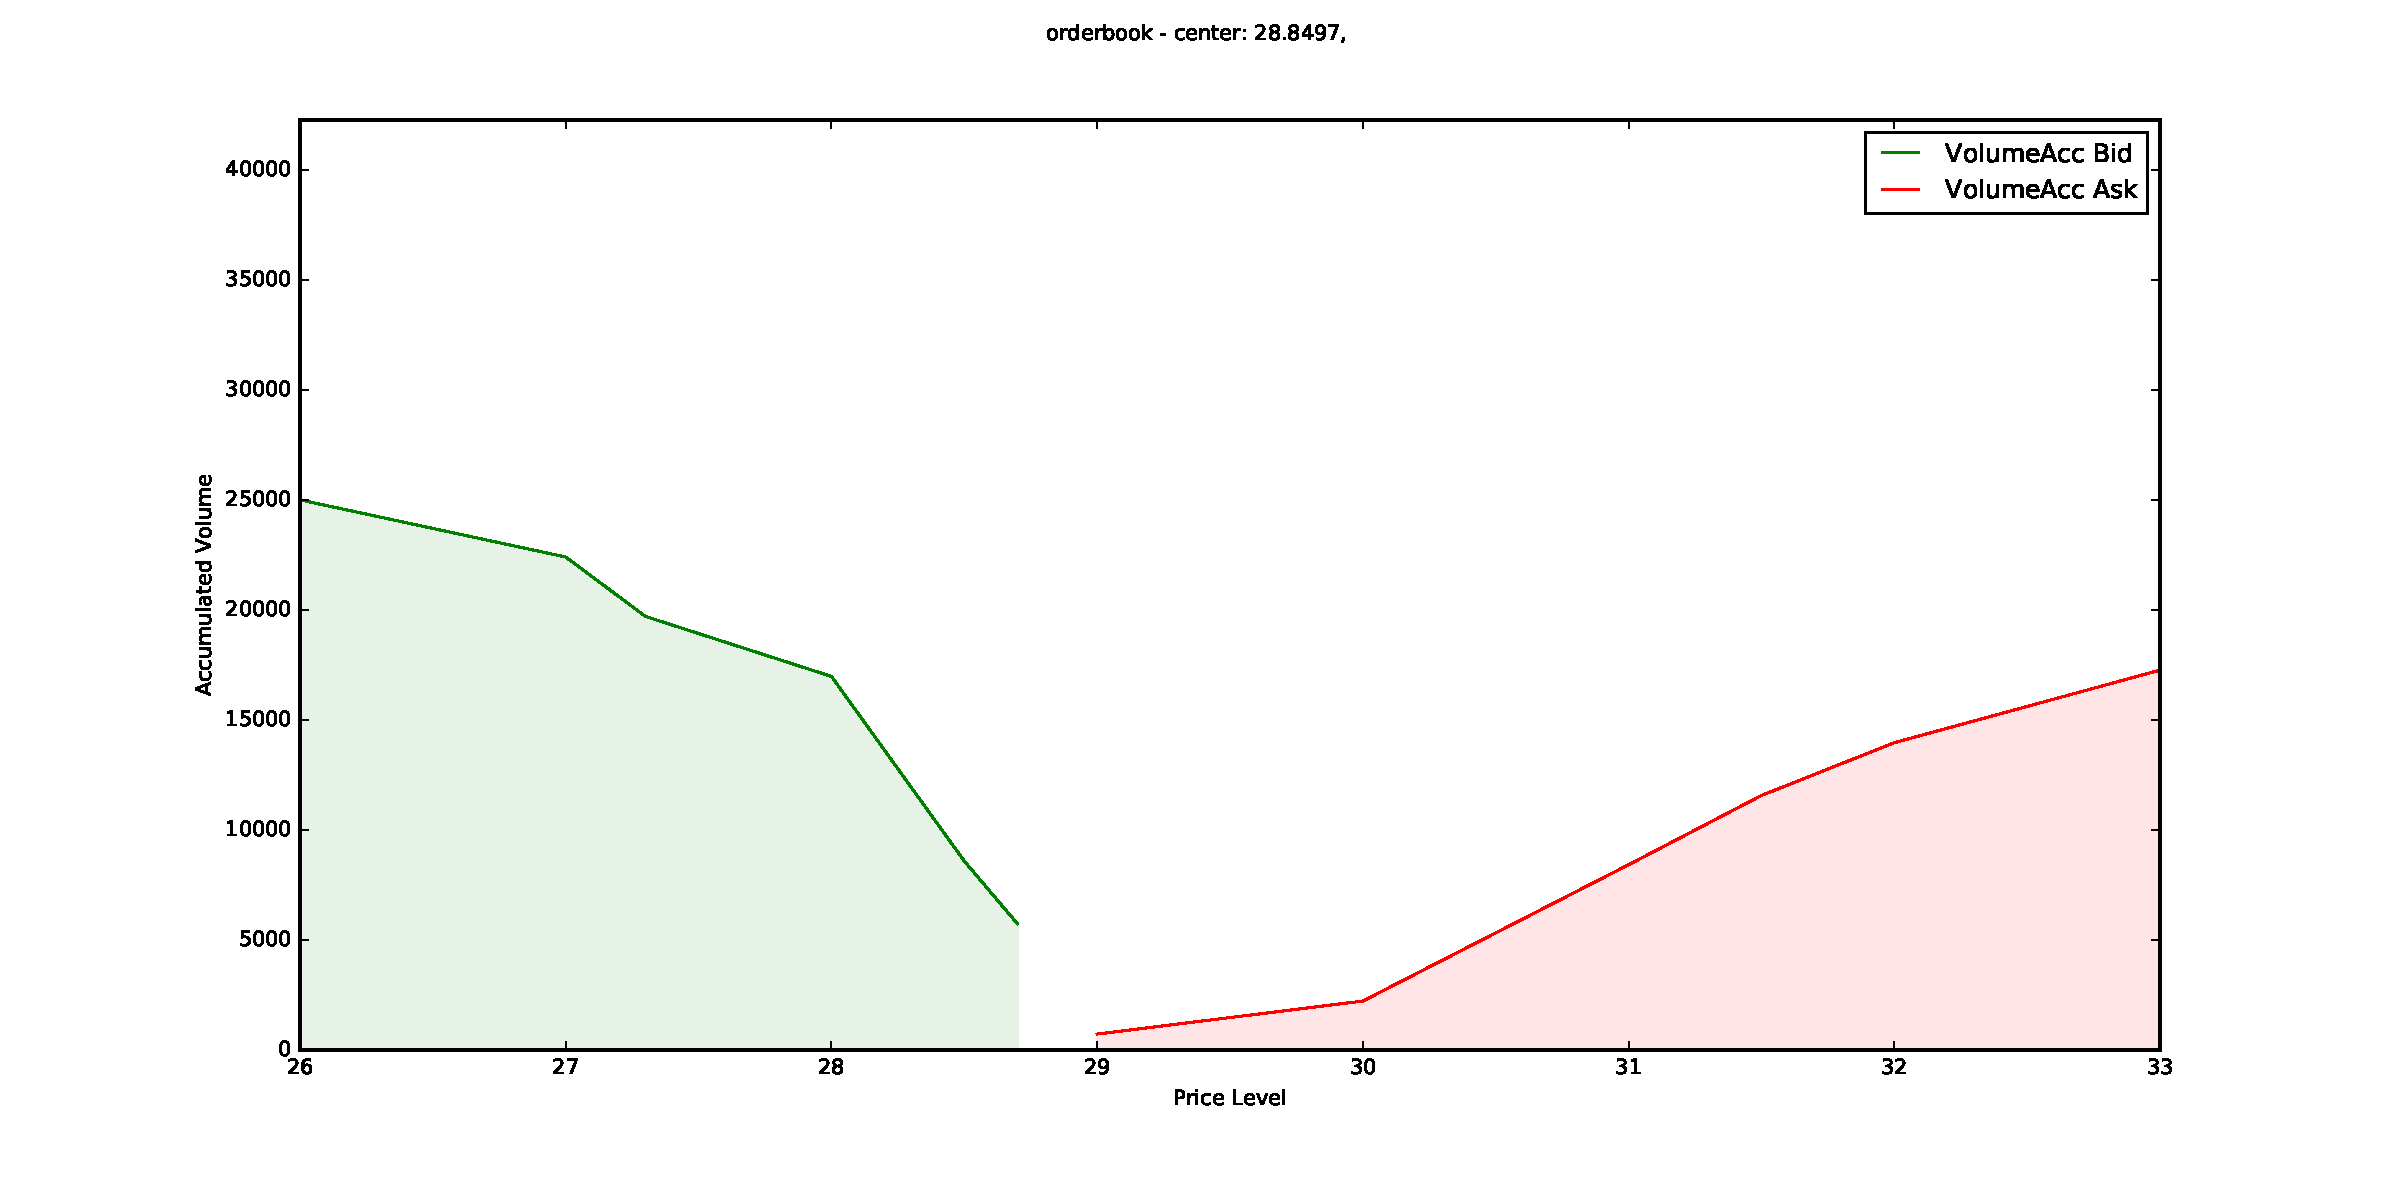
\includegraphics[width=\textwidth]{images/intro_orderbook1.pdf}
	\caption{Limit Order Book (initial)}
	\label{fig1}
\end{figure}}

\only<2>{
\begin{figure}[ht]
	\centering
   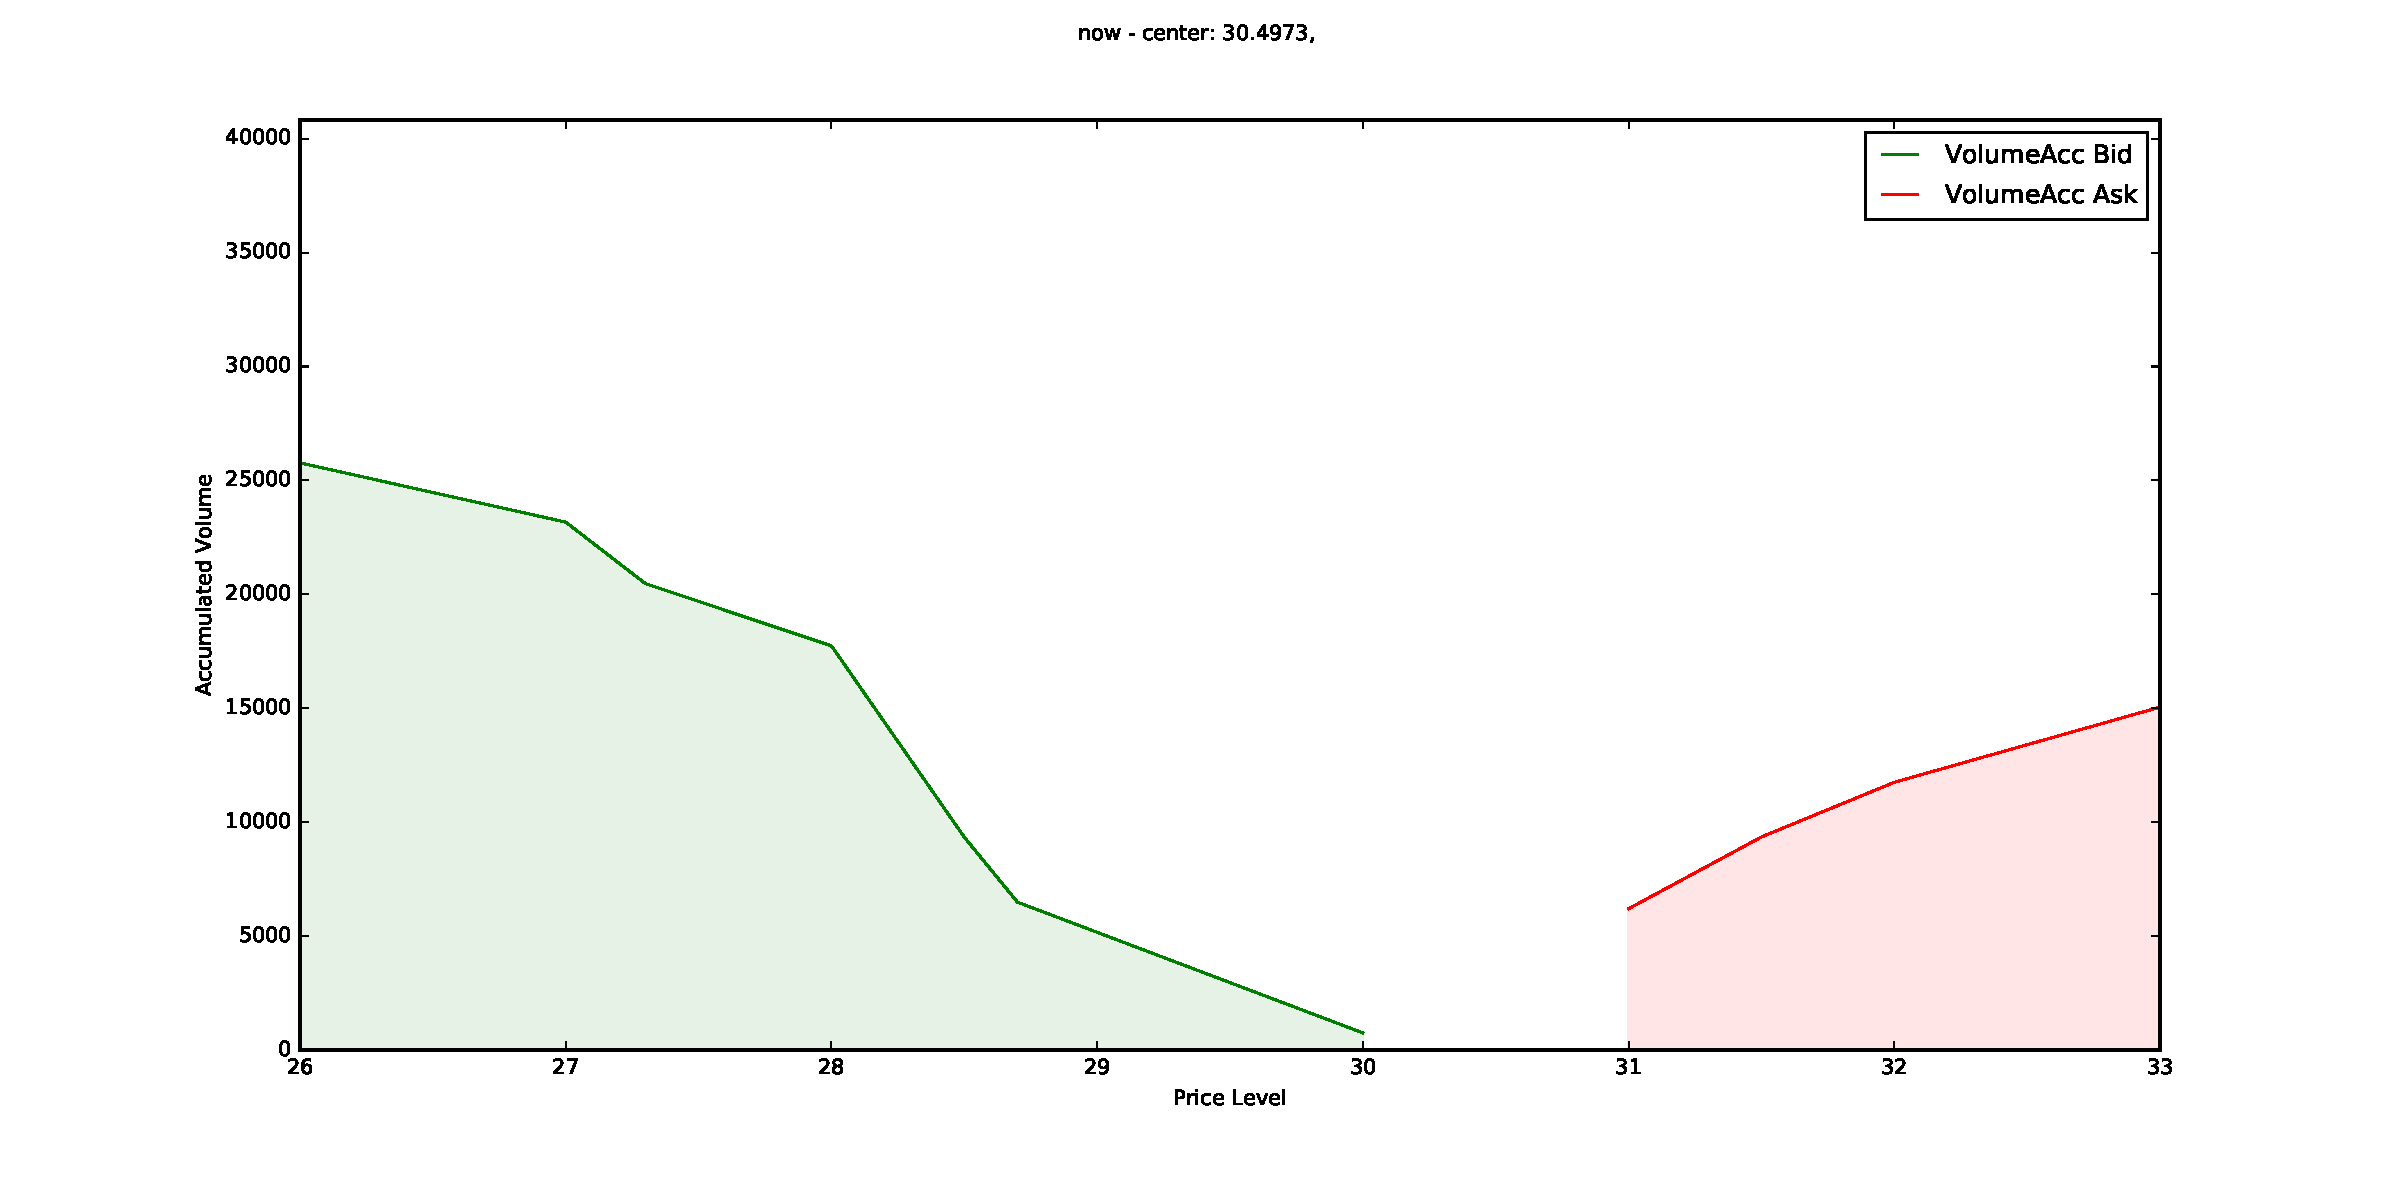
\includegraphics[width=\textwidth]{images/intro_orderbook2.pdf}
	\caption{Limit Order Book (after trade)}
	\label{fig1}
\end{figure}}

\end{frame}

\begin{frame}[fragile]{Slippage}

Placing small orders, chances are high to get a good price. Larger orders \emph{eat} into the book and are fulfilled at successively worse price levels.

\scalebox{0.6}{
\begin{tabular}{lrlrrr}
\toprule
{} &  Amount &    Type &  Volume &  VolumeAcc &  norm\_Price \\
\midrule
28.00 &   300.0 &     bid &  8400.0 &    16990.0 &    0.970546 \\
28.50 &   100.0 &     bid &  2850.0 &     8590.0 &    0.987877 \\
28.70 &   200.0 &     bid &  5740.0 &     5740.0 &    0.994810 \\
28.85 &     NaN &  center &     NaN &        NaN &         NaN \\
29.00 &    25.0 &     ask &   725.0 &      725.0 &    1.005208 \\
30.00 &    50.0 &     ask &  1500.0 &     2225.0 &    1.039871 \\
31.00 &   200.0 &     ask &  6200.0 &     8425.0 &    1.074533 \\
\bottomrule
\end{tabular}}

\scalebox{0.7}{
\begin{tabular}{l|l|r}
20 shares: & 150 shares: & 500 shares\\
\hline
Buy 20 @ 29 & Buy 25 @ 29\$ & Buy 25 @ 29\$\\
& Buy 50 @ 30\$ & Buy 50 @ 30\$\\
& Buy 75 @ 31\$ & Buy 200 @ 31\$\\
& & Buy 100 @ 31.50\$ \\
& & Buy 75 @ 32\$\\
& & Buy 50 @ 33\$\\
\hline
580\$ & 4,549.50\$ & 15,625\$\\
\hline
Avg: 29\$ & Avg: 30.33\$ & Avg: 31.25\$\\
Slippage: 0.00\$ & Slippage 1.33 \$ & Slippage 2.25 \$ \\
Cost: 0.00\$ & Cost 200 \$ & Cost 1,125 \$
\end{tabular}}
\end{frame}


\begin{frame}[fragile]{Order strategy: Submit and Leave Strategy}
\begin{overlayarea}{\textwidth}{14\baselineskip}

Scenario: You want to buy 100 shares of AIWC within the next 2 hours.
Solution: Place a limit order at t=0: BUY 100 @29.5\$
\vspace{2mm}

\only<1>{
\scalebox{0.6}{
\begin{tabular}{lrlrrr}
\toprule
{} &  Amount &    Type &  Volume &  VolumeAcc &  norm\_Price \\
\midrule
28.00 &   300.0 &     bid &  8400.0 &    16990.0 &    0.970546 \\
28.50 &   100.0 &     bid &  2850.0 &     8590.0 &    0.987877 \\
28.70 &   200.0 &     bid &  5740.0 &     5740.0 &    0.994810 \\
28.85 &     NaN &  center &     NaN &        NaN &         NaN \\
\color{red}29.00 &    \color{red}25.0 &     \color{red}ask &   \color{red}725.0 &      \color{red}725.0 &    \color{red}1.005208 \\
30.00 &    50.0 &    ask &  1500.0 &     2225.0 &    1.039871 \\
31.00 &   200.0 &     ask &  6200.0 &     8425.0 &    1.074533 \\
\bottomrule
\end{tabular}}
\vspace{2mm}

{\color{red}25} shares fall in your bid limit and are matched immediately (at t=0).}


\only<2>{
\scalebox{0.6}{
\begin{tabular}{lrlrrr}
\toprule
{} &  Amount &    Type &  Volume &  VolumeAcc &  norm\_Price \\
\midrule
28.50 &   100.0 &     bid &  2850.0 &    10802.5 &    0.958006 \\
28.70 &   200.0 &     bid &  5740.0 &     7952.5 &    0.964729 \\
\color{mygreen}29.50 &    \color{mygreen}75.0 &     \color{mygreen}bid &  \color{mygreen}2212.5 &     \color{mygreen}2212.5 &    \color{mygreen}0.991620 \\
29.75 &     NaN &  center &     NaN &        NaN &         NaN \\
30.00 &    50.0 &     ask &  1500.0 &     1500.0 &    1.008427 \\
31.00 &   200.0 &     ask &  6200.0 &     7700.0 &    1.042041 \\
31.50 &   100.0 &     ask &  3150.0 &    10850.0 &    1.058848 \\
\bottomrule
\end{tabular}}
\vspace{2mm}


{\color{mygreen}75} shares remain as bid in the orderbook.
}

\only<3>{
\scalebox{0.6}{
\begin{tabular}{lrlrrr}
\toprule
{} &  Amount &    Type &  Volume &  VolumeAcc &  norm\_Price \\
\midrule
28.50 &   100.0 &     bid &  2850.0 &     9917.5 &    0.958006 \\
28.70 &   200.0 &     bid &  5740.0 &     7067.5 &    0.964729 \\
\color{mygreen}29.50 &    \color{mygreen}45.0 &     \color{mygreen}bid &  \color{mygreen}1327.5 &     \color{mygreen}1327.5 &    \color{mygreen}0.991620 \\
29.75 &     NaN &  center &     NaN &        NaN &         NaN \\
30.00 &    50.0 &     ask &  1500.0 &     1500.0 &    1.008427 \\
31.00 &   200.0 &     ask &  6200.0 &     7700.0 &    1.042041 \\
31.50 &   100.0 &     ask &  3150.0 &    10850.0 &    1.058848 \\
\bottomrule
\end{tabular}}
\vspace{2mm}

At t=57 Warren Buffett accepts your bid and sells you {\color{mygreen}30} shares for 29.5\$ each.

{\color{mygreen}45} shares remain as bid in the orderbook.
}

\only<4>{
\scalebox{0.6}{
\begin{tabular}{lrlrrr}
\toprule
{} &  Amount &    Type &  Volume &  VolumeAcc &  norm\_Price \\
\midrule
28.00 &   300.0 &     bid &  8400.0 &    16990.0 &    0.954159 \\
28.50 &   100.0 &     bid &  2850.0 &     8590.0 &    0.971198 \\
28.70 &   200.0 &     bid &  5740.0 &     5740.0 &    0.978013 \\
29.35 &     NaN &  center &     NaN &        NaN &         NaN \\
30.00 &     5.0 &     ask &   150.0 &      150.0 &    1.022314 \\
31.00 &   200.0 &     ask &  6200.0 &     6350.0 &    1.056391 \\
31.50 &   100.0 &     ask &  3150.0 &     9500.0 &    1.073429 \\\bottomrule
\end{tabular}}
\vspace{2mm}

At t=119 time is over. Sell all remaining shares for current market price

\begin{itemize}
\item from Alice:   $\Rightarrow 25*29\$ = 725\$$  (at t=0)
\item from Warren Buffett:   $\Rightarrow (30)*29.5\$ = 885\$$  (at t=57)
\item from Bob and Cedar:   $\Rightarrow (20+25)*30\$ = 1350\$$   (at t=119)
\end{itemize}
Total: 2960\$ (avg price: 29.6\$)

\emph{Saved 40\$ compared to Simple Market Order}}

\end{overlayarea}
\end{frame}


\begin{frame}[fragile]{Order strategy: Submit and Leave Strategy v2}
\begin{overlayarea}{\textwidth}{14\baselineskip}

\begin{itemize}
\item Place limit order, periodically (e.g. every 10 minutes) update limit, depending on trade process.
\item Increasing aggression (= accepting more slippage) towards end of period)
\item Use Reinforcement Learning to find optimal aggressiveness (=limits).
\item Exploit Market/Orderbook Features
\begin{itemize}
\item Indication of price fall or rise?!
\item More people trying to sell or to buy?!
\end{itemize}
\end{itemize}



\end{overlayarea}
\end{frame}

\section{Reinforcement Learning Approach}

\begin{frame}[fragile]{Reinforcement Learning Approach: Actions}
\begin{overlayarea}{\textwidth}{14\baselineskip}


Actions:  $a \in \mathbb{R} [-1, 1]$
\vspace{2mm}

\scalebox{0.6}{
\begin{tabular}{lrlrrr}
\toprule
{} &  Amount &    Type &  Volume &  VolumeAcc &  norm\_Price \\
\midrule
28.00 &   300.0 &     bid &  8400.0 &    16990.0 &    0.970546 \\
28.50 &   100.0 &     bid &  2850.0 &     8590.0 &    0.987877 \\
28.70 &   200.0 &     bid &  5740.0 &     5740.0 &    0.994810 \\
28.85 &     NaN &  center &     NaN &        NaN &         NaN \\
\color{mygreen}29.00 &    25.0 &     ask &   725.0 &      725.0 &    1.005208 \\
30.00 &    50.0 &     ask &  1500.0 &     2225.0 &    1.039871 \\
\color{red}31.00 &   200.0 &     ask &  6200.0 &     8425.0 &    1.074533 \\
\bottomrule
\end{tabular}}
\vspace{2mm}

Example:

current best price: {\color{mygreen}29.00\$}\\
worst price level, when buying 100 shares: {\color{red}31.00\$}\\
$a=1.00 \Rightarrow limit=31$   (i.e. simple market order)\\
$a=0.25 \Rightarrow limit=29.5$\\
$a=0.00 \Rightarrow limit=29$ (i.e. buy only for current best price)\\
$a=-1.0 \Rightarrow limit=27$\\

\end{overlayarea}
\end{frame}

\begin{frame}[fragile]{Reinforcement Learning Approach: Costs}
\begin{overlayarea}{\textwidth}{14\baselineskip}


Costs: Difference between benchmark and obtained price.
\vspace{2mm}

\scalebox{0.6}{
\begin{tabular}{lrlrrr}
\toprule
{} &  Amount &    Type &  Volume &  VolumeAcc &  norm\_Price \\
\midrule
28.00 &   300.0 &     bid &  8400.0 &    16990.0 &    0.970546 \\
28.50 &   100.0 &     bid &  2850.0 &     8590.0 &    0.987877 \\
28.70 &   200.0 &     bid &  5740.0 &     5740.0 &    0.994810 \\
28.85 &     NaN &  center &     NaN &        NaN &         NaN \\
\color{mygreen}29.00 &    25.0 &     ask &   725.0 &      725.0 &    1.005208 \\
30.00 &    50.0 &     ask &  1500.0 &     2225.0 &    1.039871 \\
31.00 &   200.0 &     ask &  6200.0 &     8425.0 &    1.074533 \\
\bottomrule
\end{tabular}}
\vspace{2mm}

Example:

current best price: {\color{mygreen}29.00\$} (benchmark: $29\$ * 100 = 2900\$$)

\begin{itemize}
\item $25*29\$ = 725\$$  (at t=0), costs=0
\item $30*29.5\$ = 885\$$  (at t=57), costs = $30*0.5 \Rightarrow 15\$$
\item $(20+25)*30\$ = 1350\$$   (at t=119), costs = $45*1.0 \Rightarrow 45\$$
\end{itemize}
Total: 2960\$,  Acc Costs: 60\$

\end{overlayarea}
\end{frame}

\begin{frame}[fragile]{Reinforcement Learning Approach: States}
\begin{overlayarea}{\textwidth}{14\baselineskip}


States:  [private variables + market variables]
\vspace{2mm}

\scalebox{0.6}{
\begin{tabular}{lrlrrr}
\toprule
{} &  Amount &    Type &  Volume &  VolumeAcc &  norm\_Price \\
\midrule
28.00 &   300.0 &     bid &  8400.0 &    16990.0 &    0.970546 \\
28.50 &   100.0 &     bid &  2850.0 &     8590.0 &    0.987877 \\
28.70 &   200.0 &     bid &  5740.0 &     5740.0 &    0.994810 \\
28.85 &     NaN &  center &     NaN &        NaN &         NaN \\
\color{mygreen}29.00 &    25.0 &     ask &   725.0 &      725.0 &    1.005208 \\
30.00 &    50.0 &     ask &  1500.0 &     2225.0 &    1.039871 \\
\color{red}31.00 &   200.0 &     ask &  6200.0 &     8425.0 &    1.074533 \\
\bottomrule
\end{tabular}}
\vspace{2mm}

Private Variables:
\begin{itemize}
\item Time left (t=119, 118, ..., 0)
\item Volume left (vol=100, 75, 37.8, ..., 0)
\end{itemize}

Market Variables:
\begin{itemize}
\item Bid-Ask Spread
\item Bid-Ask Volume Misbalance
\item current market price
\item ... research topic ...
\end{itemize}

\end{overlayarea}
\end{frame}

\begin{frame}[fragile]{Reinforcement Learning Approach: Algorithm}
\begin{overlayarea}{\textwidth}{14\baselineskip}

\begin{itemize}
\item Q-Learning
\item Q Function Approximation: (1 layer NN with 64 neurons)
\item Replay Memory
\end{itemize}

\end{overlayarea}
\end{frame}



\section{Technical Background}

\begin{frame}[fragile]{Data Origination}
\begin{overlayarea}{\textwidth}{14\baselineskip}
  Data fetched from Poloniex Bitcoin Market Place via HTTP GET request:
  
  \footnotesize{Call \url{https://poloniex.com/public?command=returnOrderBook&currencyPair=USDT_BTC&depth=5000}}

  \begin{lstlisting}[frame=single, breaklines=true, basicstyle=\footnotesize, belowskip=-1.0 \baselineskip]
{"asks":[["705.450000",2.772181],["706.170000",0.052838], ... ], "bids":[["705.000000",0.158232],["703.700000",0.001250], ... ], "isFrozen": 0, "seq": 63413296}  \end{lstlisting}
\only<2>{
\noindent\begin{minipage}{0.45\textwidth}
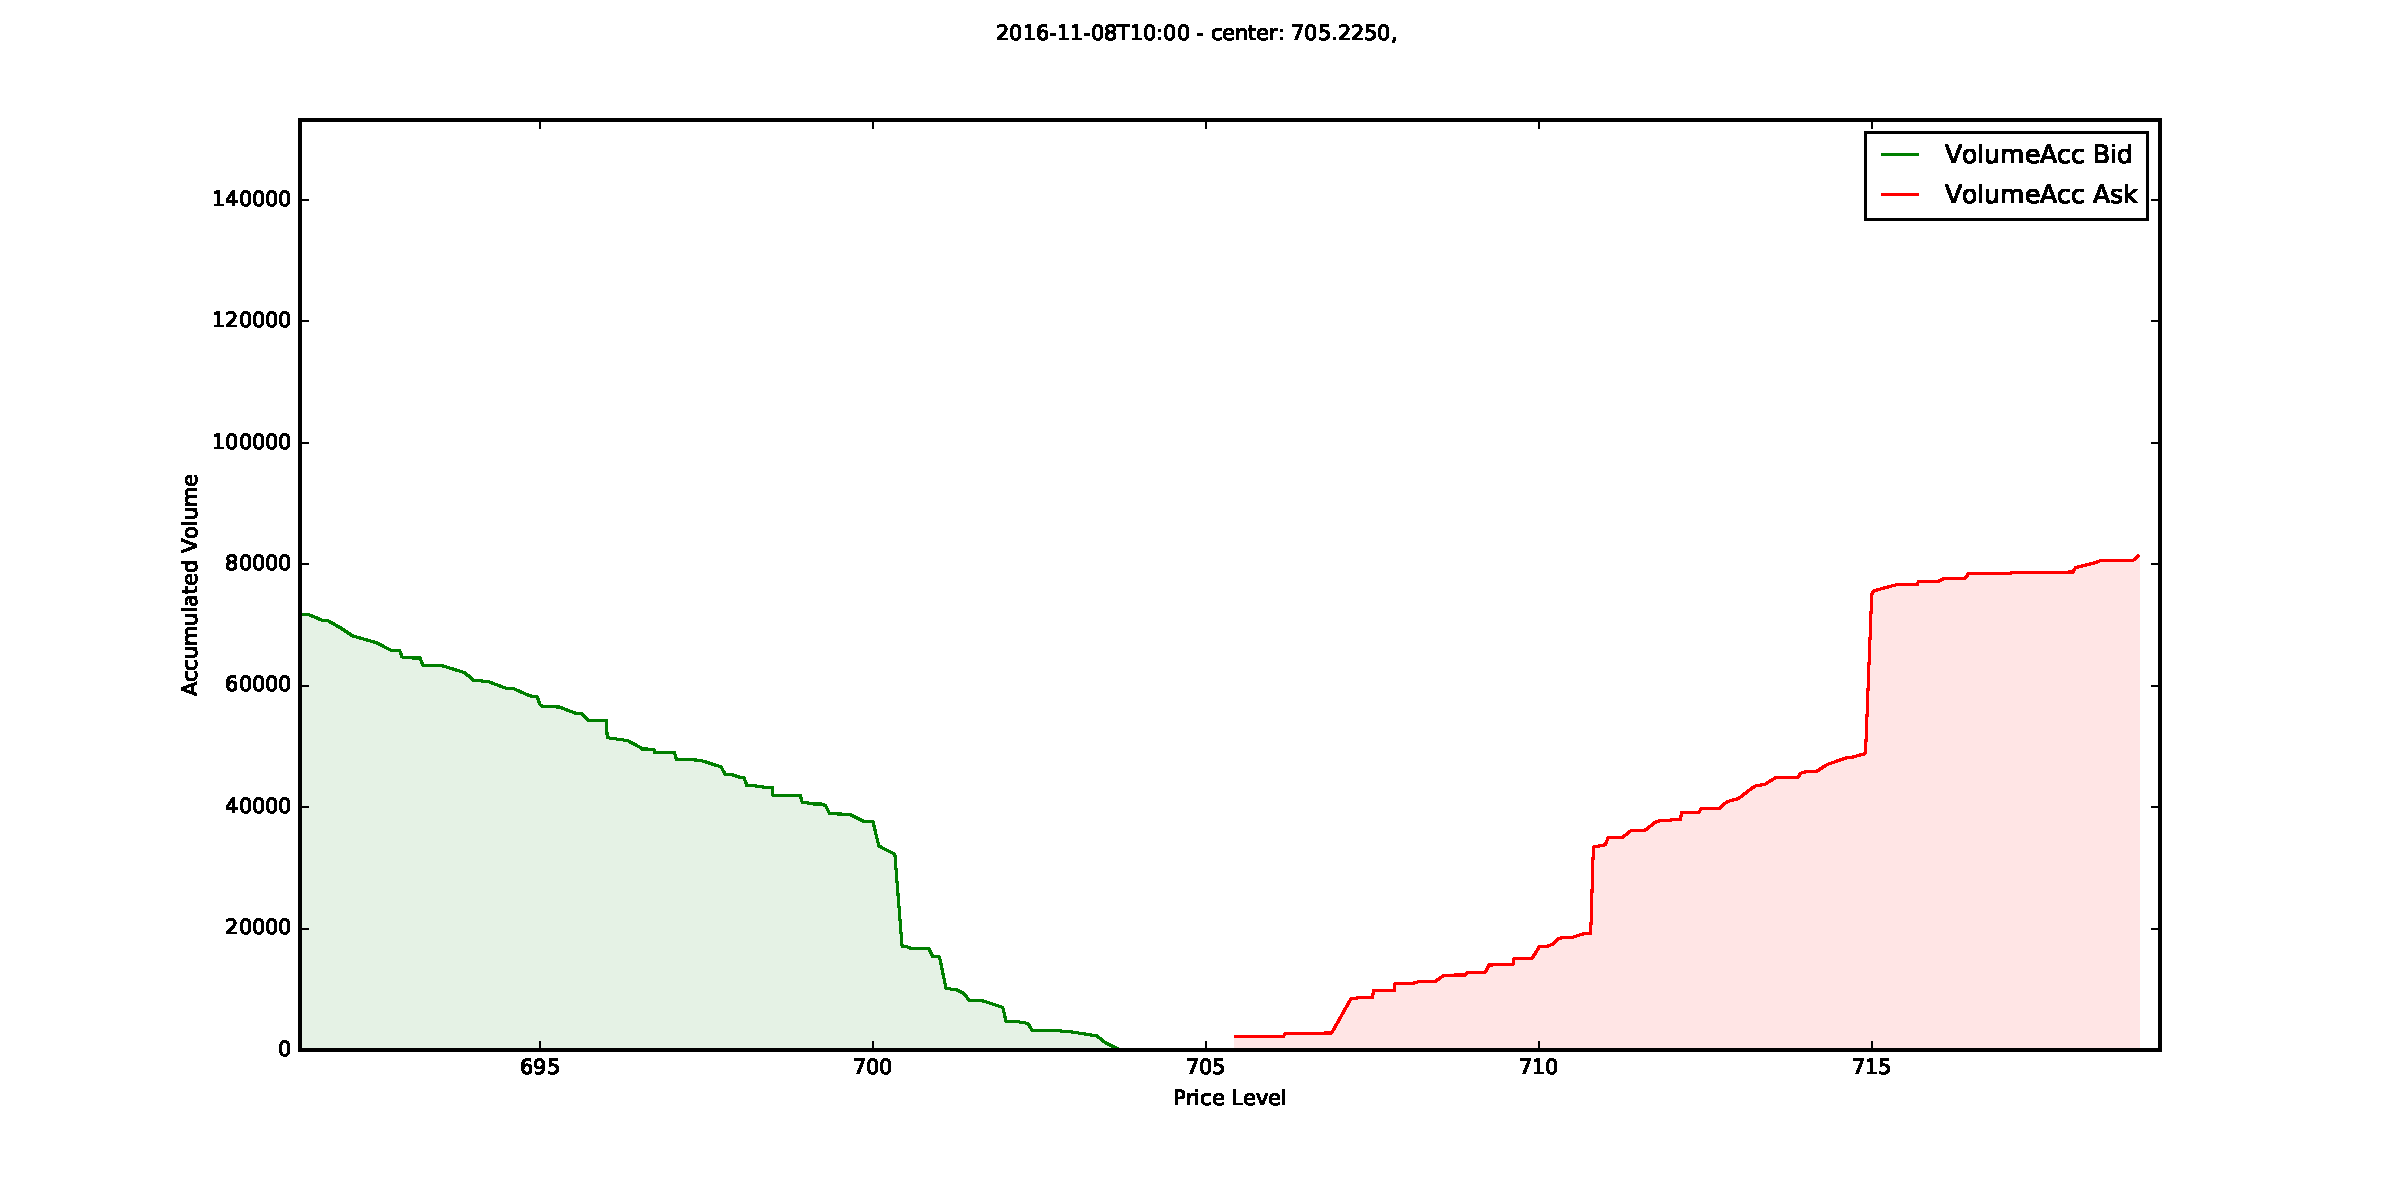
\includegraphics[width=\textwidth]{images/orderbook_sample2}
\end{minipage}%
\begin{minipage}{0.55\textwidth}\raggedleft
\begin{itemize}
\item 9 Currencypairs: \lstinline[basicstyle=\scriptsize]{'USDT_BTC', 'BTC_ETH', 'BTC_XMR', 'BTC_XRP', 'BTC_FCT', 'BTC_NAV', 'BTC_DASH', 'BTC_MAID', 'BTC_ZEC'}
\item Frequency: 1 per Minute since 2016-11-08T10:00
\item Datasize: \textasciitilde290KB per full query
\item2.8GB for 109,582\footnote{as per 2017-01-23T13:36} snapshots of USDT\_BTC
\end{itemize}
\end{minipage}}
\end{overlayarea}
\end{frame}

\begin{frame}[fragile]{Data Preprocessing}

  \lstinline{manage_orderbooks.py} $\Rightarrow$ \lstinline{extract_orderbooks_for_one_currencypair}
  \begin{itemize}
  \item one file per currencypair, one line per minute
  \item round and aggregate similar pricelevels:   
  \[ 2.87 * 873.00 =
  \begin{cases}
    0.34 * 873.00000122\\
    2.53 * 873.00000121\\
  \end{cases}
\]
  \item Note: Bitcoins can be split into arbitrarily small chunks. In contrast it is usually not possible to buy 1.76 shares of stocks like AIWC.
  \item Conversion to custom class \lstinline{OrderbookContainer}
  \end{itemize}
    
\end{frame}

\begin{frame}[fragile]{Orderbook Container}

Implemented in Python
\begin{lstlisting}[frame=single, breaklines=true, basicstyle=\scriptsize, belowskip=-1.0 \baselineskip]
ob=OrderbookContainer(timestamp="2016-11-08T10:00",
                      bids=pd.DataFrame([200,100,300],
                        columns=['Amount'], index=[28.7,28.5,28]),
                      asks=pd.DataFrame([25,50,200],
                        columns=['Amount'], index=[29,30,31]))
                        
# Available methods
ob.plot(outfile='sample.pdf')  # plt.show or plt.savefig
ob.asks  # pd.DataFrame
ob.bids  # pd.DataFrame
ob.get_ask()  # float
ob.get_current_price(volume=100)  # float
ob.enrich()  # Adds Volume, VolumeAcc and norm_Price
ob.head(depth=3)  # pd.DataFrame
\end{lstlisting}

\scalebox{0.6}{
\begin{tabular}{lrlrrr}
\toprule
{} &  Amount &    Type &  Volume &  VolumeAcc &  norm\_Price \\
\midrule
28.00 &   300.0 &     bid &  8400.0 &    16990.0 &    0.970546 \\
28.50 &   100.0 &     bid &  2850.0 &     8590.0 &    0.987877 \\
28.70 &   200.0 &     bid &  5740.0 &     5740.0 &    0.994810 \\
28.85 &     NaN &  center &     NaN &        NaN &         NaN \\
29.00 &    25.0 &     ask &   725.0 &      725.0 &    1.005208 \\
30.00 &    50.0 &     ask &  1500.0 &     2225.0 &    1.039871 \\
31.00 &   200.0 &     ask &  6200.0 &     8425.0 &    1.074533 \\
\bottomrule
\end{tabular}}
  
\end{frame}

\begin{frame}[fragile]{Orderbook Windows (1)}

\begin{figure}[ht]
	\centering
   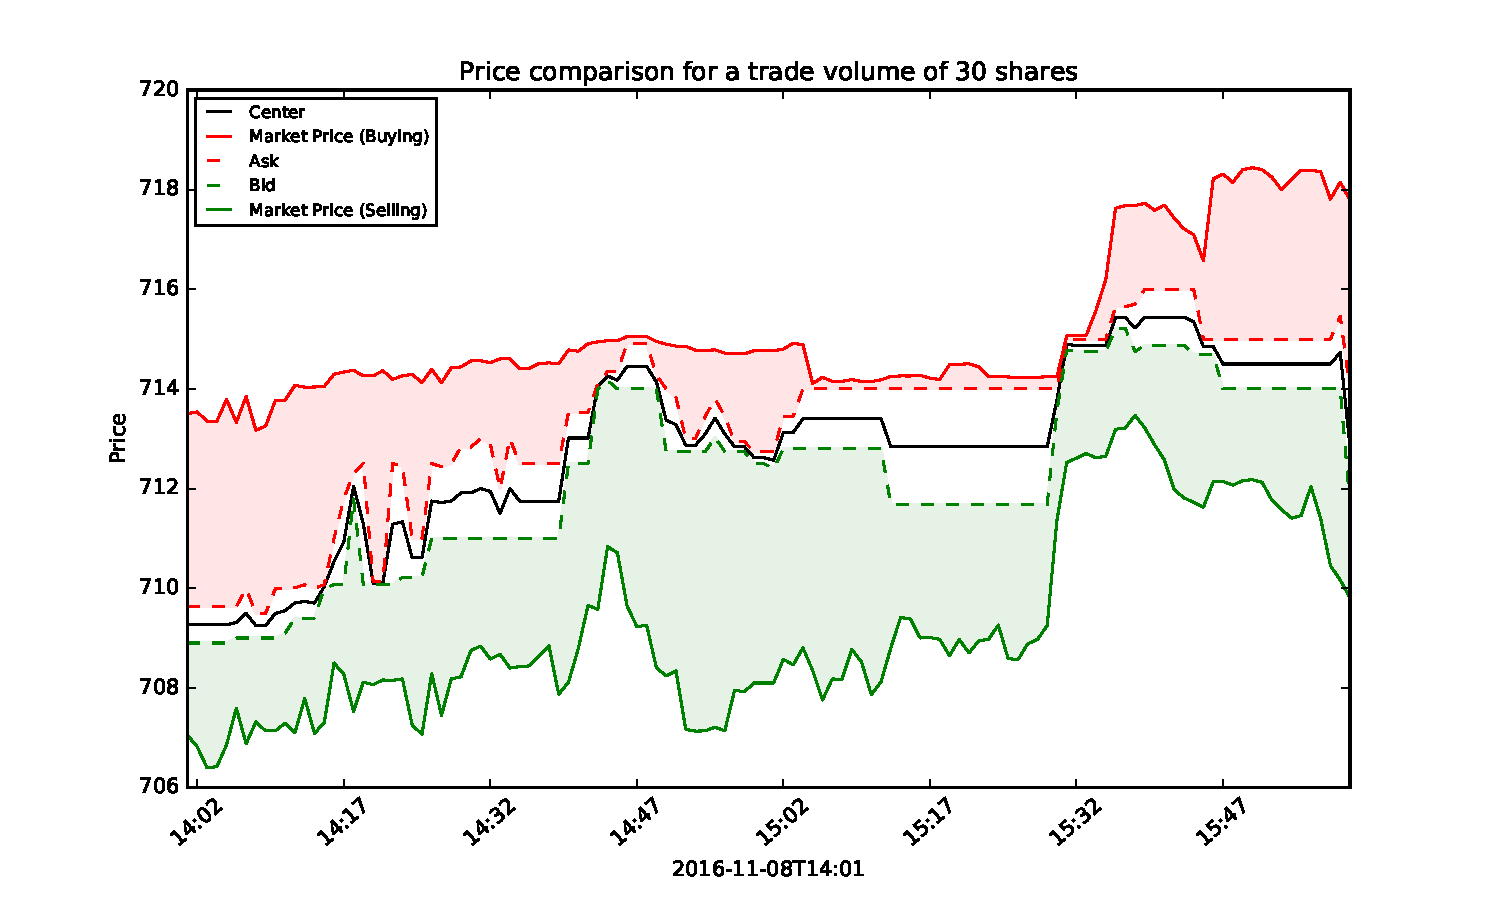
\includegraphics[width=0.9\textwidth]{images/episode_window2.pdf}
	\caption{Episode Window over 120 minutes (increasing prices)}
	\label{fig1}
\end{figure}

Ideal: Moderat or negativ aggression in early window. Aggressiv towards end of window

\end{frame}

\begin{frame}[fragile]{Orderbook Windows (2)}

\begin{figure}[ht]
	\centering
   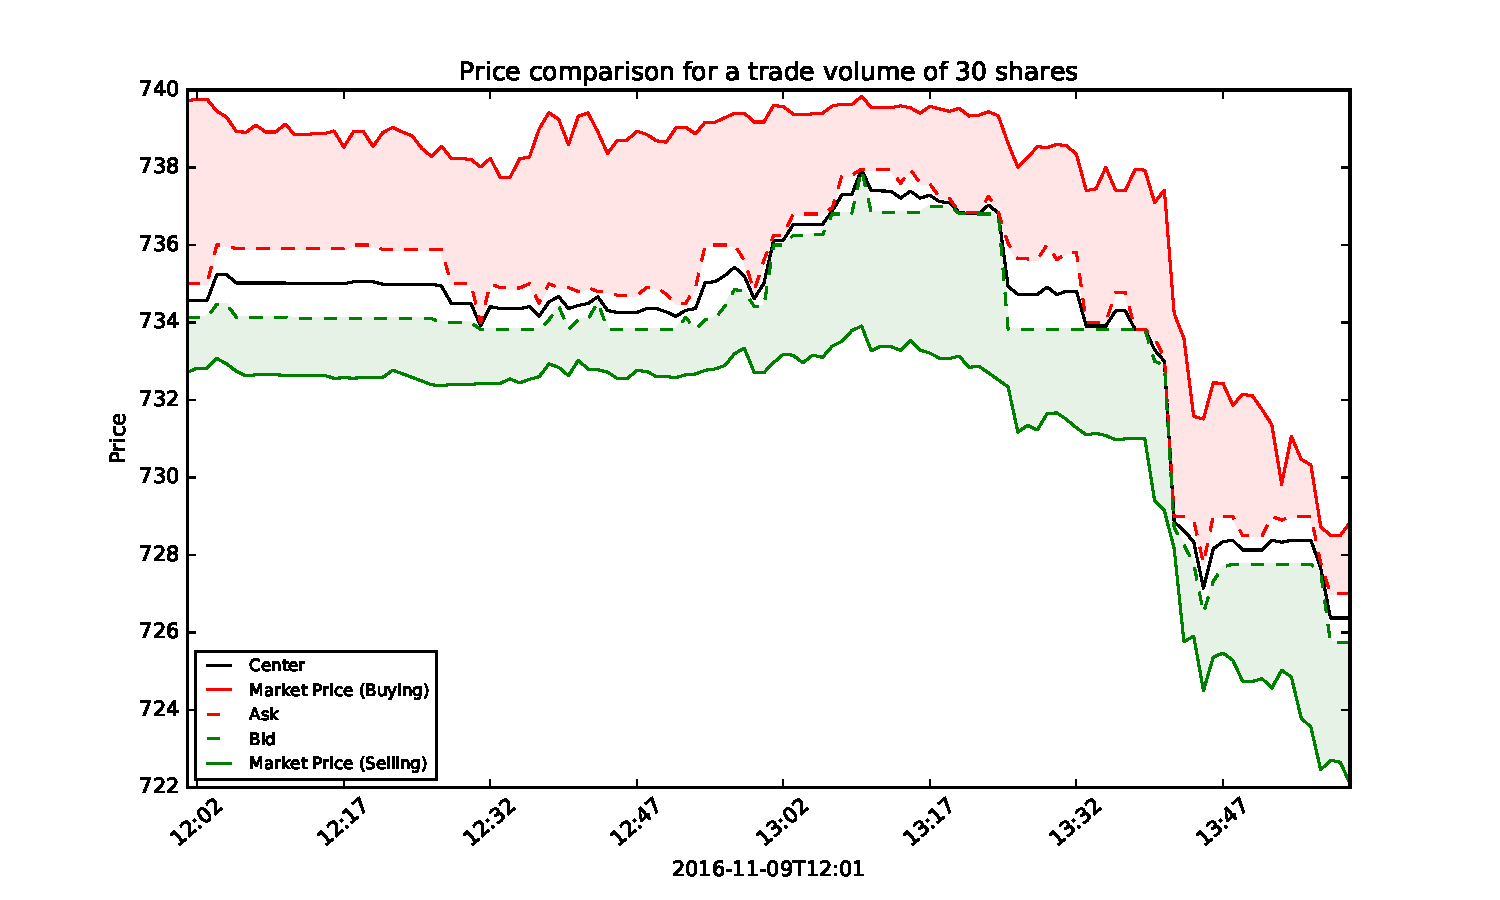
\includegraphics[width=0.9\textwidth]{images/episode_window13.pdf}
	\caption{Episode Window over 120 minutes (decreasing prices)}
	\label{fig1}
\end{figure}

Ideal: Moderat aggression in early window. Try everything to finish trade before the price drops.

\end{frame}


\begin{frame}[fragile]{Orderbook Trade Simulator}

\begin{lstlisting}[frame=single, breaklines=true, basicstyle=\scriptsize, belowskip=-1.0 \baselineskip]
vol = 20
T   = 12
P   = 10
ots = OrderbookTradingSimulator(volume=vol, tradingperiods=T, decisionfrequency=P)
for e in range(T):
    action=0.4
    res = ots.trade(orderbooks=episode_windows[2][P*e:P*(e+1)], agression_factor=action)
    
display(ots.history)
\end{lstlisting}

\scalebox{0.44}{
\begin{tabular}{lrrrrrrrrrrrrlrrrr}
\toprule
{} &  a &     ASK &     BID &      CENTER &    LIMIT &  SPREAD &     VOLUME &        avg &     cashflow &       cost &  cost\_avg & forced &    high &     low &  traded &  LIMIT\_MAX \\
\midrule
14:01 &     0.4 &  709.63 &  708.90 &  709.26 &  711.634 &    0.73 &  20.00 &  710.22 & -5374.46 &   4.52 &   0.59 &  False &  711.61 &  709.50 &       7.567243 &     714.64 \\
14:11 &     0.4 &  710.66 &  709.10 &  709.87 &  712.120 &    1.56 &  12.43 &  711.79 & -1810.06 &   5.49 &   2.16 &  False &  712.12 &  710.01 &       2.542967 &     714.31 \\
14:21 &     0.4 &  711.49 &  710.07 &  710.77 &  712.618 &    1.42 &   9.88 &  712.40 & -6641.97 &  25.88 &   2.77 &  False &  712.50 &  711.49 &       9.323293 &     714.31 \\
14:31 &     0.4 &  713.00 &  711.00 &  711.99 &  713.000 &    2.00 &   0.56 &  713.00 &  -403.91 &   1.90 &   3.37 &  False &  713.00 &  713.00 &       0.566497 &     713.00 \\
\bottomrule
\end{tabular}
}

\begin{itemize}
\item 12 Decision points (update of limit possible)
\item timespan of 10 minutes
\end{itemize}

\end{frame}

\section{Roadmap}
\begin{frame}[fragile]{Roadmap: General Ideas}

\begin{itemize}
\item Buying without limit (= Market Order) is costly, but fast.
\item Setting a limit does not guarantee trade fulfillment
\item Idea: Define trading period (e.g. 120 minutes)

\begin{itemize}
\item Place limit order, periodically (e.g. every 10 minutes) adapt limit
\item Early Trading period: Careful order limits (avoid slippage)
\item End of Trading period: Aggressiv order limits (accept more slippage)
\item Must trade all remaining shares at t=120 (no matter how poor the price)
\end{itemize}

\item Use Reinforcement Learning to find optimal aggressiveness (=limits).
\item Exploit Market/Orderbook Features
\begin{itemize}
\item Indication of price fall or rise?!
\item More people trying to sell or to buy?!
\end{itemize}

\end{itemize}

\end{frame}

\begin{frame}[fragile]{Roadmap: Implementation}

\begin{itemize}
\item[\checkmark] Collect data 
\item[\checkmark] Implement OrderbookContainer
\item[\checkmark] Implement OrderTradeSimulator
\item[\qed] Train RL-Agent on repeating data window
\begin{itemize}
\item[\checkmark] Actions: limit = $ask +  a | a \in [..., -1, 0, 1, ...]$
\item[\checkmark] Costs: Slippage as from initial \emph{ask}
\item[\checkmark] States: [Remaining time, Remaining Volume]
\item[\qed] Find optimal Q function for this data window
\item[\qed] Learned strategy must have small costs
\end{itemize}
\item[\qed] Train RL-Agent on various, non-overlapping data windows
\begin{itemize}
\item[\qed] Expand State dimension: spread, ask-bid-ratio, ...
\end{itemize}
\item[\qed] Train RL-Agent on various currencypairs/stocks simultaneously
\end{itemize}

\end{frame}

\begin{frame}[standout]
  Questions?
\end{frame}

\appendix

\begin{frame}[allowframebreaks]{References}

  \bibliography{demo}
  \bibliographystyle{abbrv}

\end{frame}

\end{document}
